\section{4D vertex reconstruction}
\label{VtxImp}
%editors: L. Gray & J. Bendavid

%%%*** Description of the 4D vertexing as in TP ***
%%% TTF - The text bolow is adapted from the TP, and with reference to the TP where relevant
%% TEXT ADAPTED FROM THE TP
Vertex reconstruction in the $tz$-plane, i.e. in time and position along the beam line, was studied using a time-aware extension of the deterministic annealing technique adopted in vertex reconstruction by the CMS experiment~\cite{Chatrchyan:2014fea}.  Since this technique can be extended to more than three dimensions, it is the natural choice for finding vertices in the dense environment of 200 pileup events.  
As outlined in Chapter 1 (Fig.~\ref{fig:4Dvertex_200}), the
introduction of  time information significantly improves the
performance of the vertex reconstruction algorithm in associating
tracks with vertices. For example, instances of vertex merging are
reduced from 15\% in space to 1\% in space-time, at 200 PU. 
%%P<Can this be shown for the current vertex reconstruction?
Moreover, the space-time reconstruction capability has dramatic
impact on several observables (e.g., pileup jet ID, \MET{}, b tagging,
lepton isolation), as further discussed in the next sections. 

This reconstruction method is further extended to associate the
individual photons reconstructed in the calorimeters to a collision
vertex.  The neutral particle is assigned a straight trajectory with
time-of-flight timing corrections corresponding to the $z$-vertex
positions.  This generates a set of compatible vertices, which are a
function of the time-of-flight and vertex $t_0$ information.  As
discussed in the MTD Technical Proposal~\cite{TP}, this capability
opens several possibilities, including an improved identification of
the diphoton vertex in \HGG{} decays, improved sensitivity to
long-lived particles decaying into photons, improved measurement of
the particle isolation from electromagnetic deposits, and improved
resolution in the calorimetric missing transverse energy. 

At momenta below a few GeV, the difference in time of flight between pions, kaons, and protons or heavier nuclear fragments becomes significant with respect to the time resolution of the detector.  In order to address this, the 4D vertex reconstruction is carried out in two stages.  In the first stage, the pion mass hypothesis is used to compute the time of each track at the beamline, but the uncertainty assigned to this measurement is inflated by adding in quadrature the difference in time of flight between the pion and proton mass hypothesis.  After this initial reconstruction, the compatibility of tracks with the reconstructed vertices is tested in the z-t plane under the kaon and proton mass hypotheses in addition to the nominal pion hypothesis.  Tracks which are well identified as pions, kaons or protons have the additional contribution from the mass hypothesis ambiguity removed from the uncertainty assigned to their time measurement, and those identified as kaons or protons have their time measurement at the beamline recomputed as appropriate.  These recomputed timestamps and uncertainties are then used to run the 4D vertex reconstruction a second time.

As a validation of this step Fig.~\ref{fig:tofpid_probability} reports the output probability of the particle identification step for generator matched kaons and protons. This plot shows also that for high momentum track the particle identification step is irrelevant for vertexing purposes.

\begin{figure}[!hbtp]
\centering
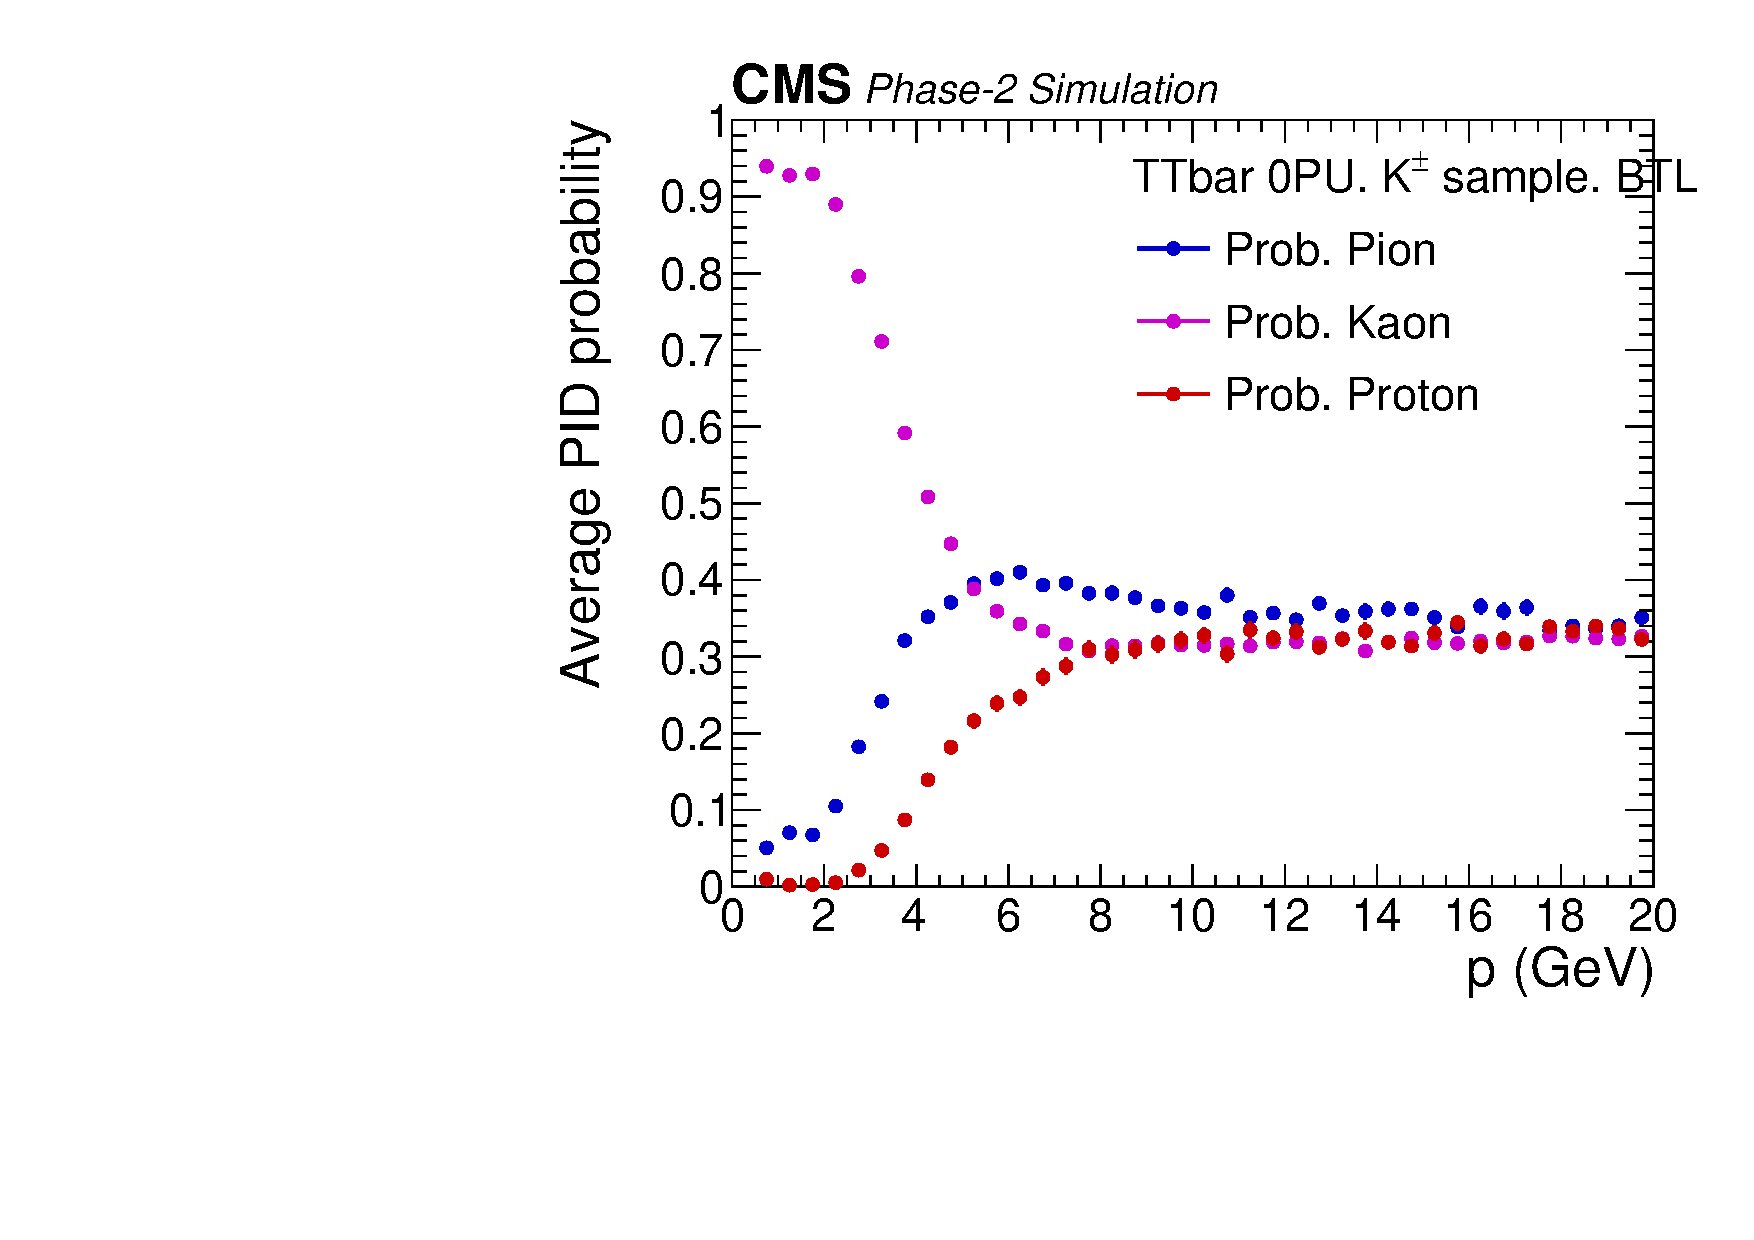
\includegraphics[width=0.48\textwidth]{fig/performance/4dvtx/kaons_PID_prob_vs_p_BTL.pdf}
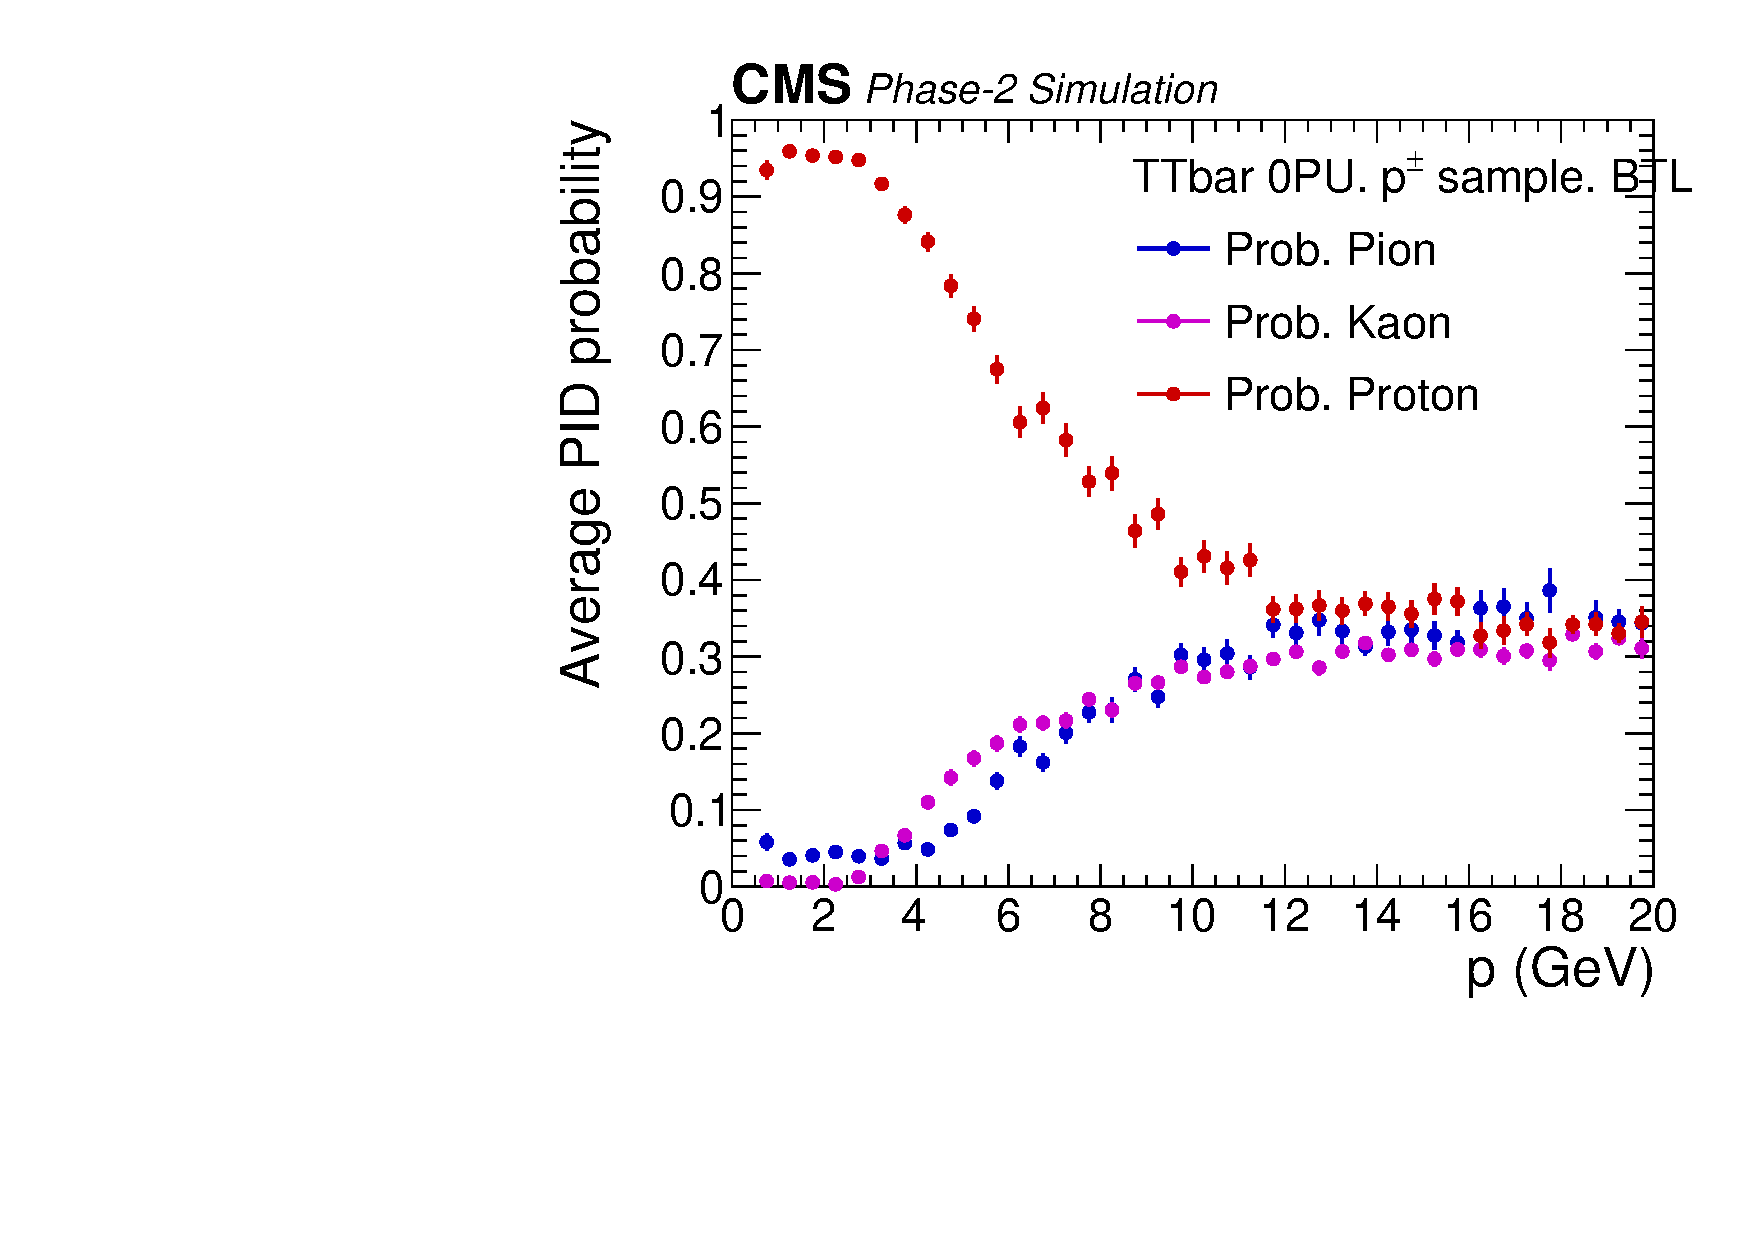
\includegraphics[width=0.48\textwidth]{fig/performance/4dvtx/protons_PID_prob_vs_p_BTL.pdf}
\caption{Probability for gen-matched kaons (left) and protons (right) to be assigned  different particle hypothesis as a function of track momentum. Tracks from TTBar events at no pile-up are used.}
\label{fig:tofpid_probability}
\end{figure}

The time resolution of the 4D vertex reconstruction for $t\bar t$ events with 200 PU is shown in Fig.~\ref{fig:vtxdtgen}.  To further validate the particle identification step, the reconstructed time before and after the particle ID step is compared to the generated time of the hard interaction for tracks reconstructed within $|\Delta z|<1$~mm of the generated hard interaction, with the results in Fig.~\ref{fig:pidtres} showing a significant reduction in the tails of the distribution as expected.

\begin{figure}[!hbtp]
\centering
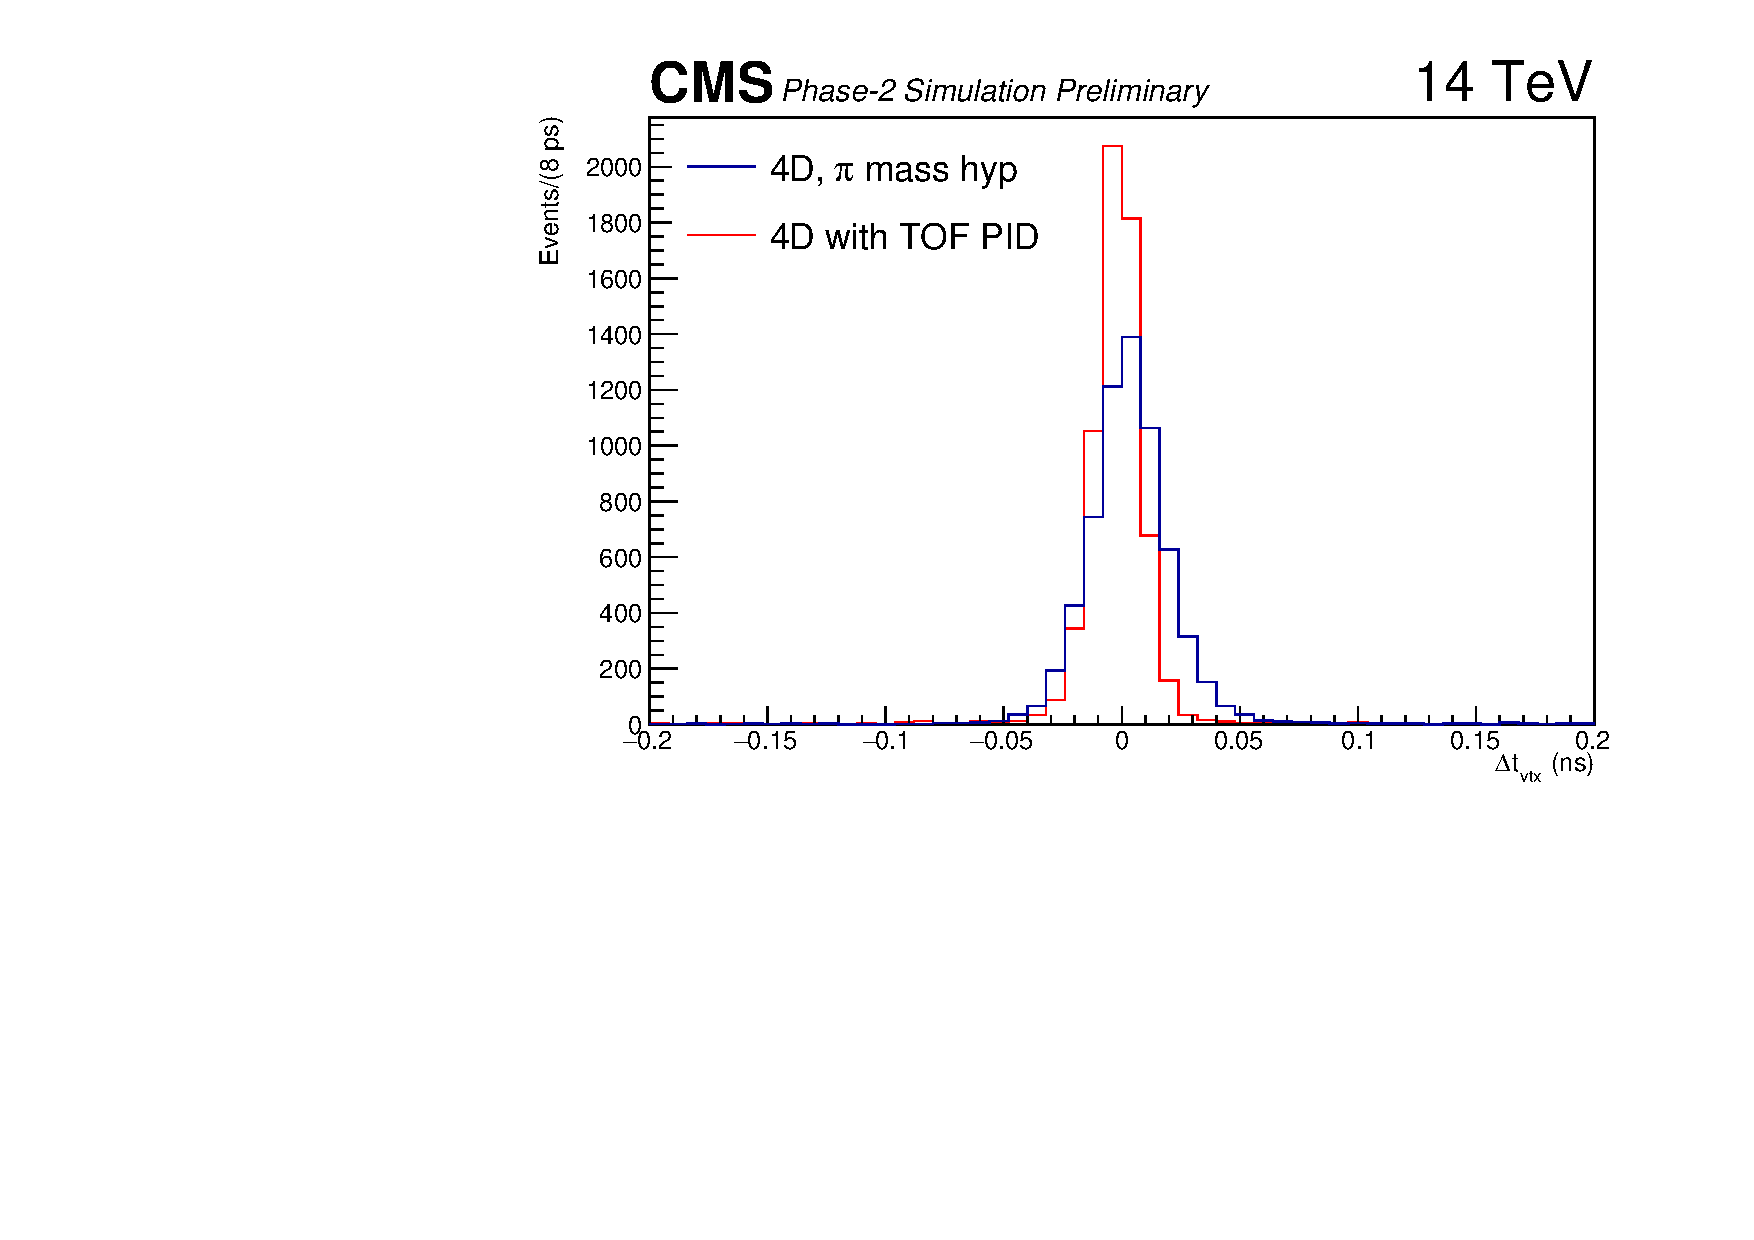
\includegraphics[width=0.48\textwidth]{fig/performance/4dvtx/ttbarpu200/dtvtxgen_pu200_prelim.pdf}
\caption{Reconstructed time of the first vertex in the collection compared to the generated time of the hard interaction for the first step of the 4d vertex reconstruction using the pion mass hypothesis, and the second step incorporating the time-of-flight particle identification.  The core of the distribution for the second step corresponds to a resolution of approximately 10~ps.}
\label{fig:vtxdtgen}
\end{figure}

\begin{figure}[!hbtp]
\centering
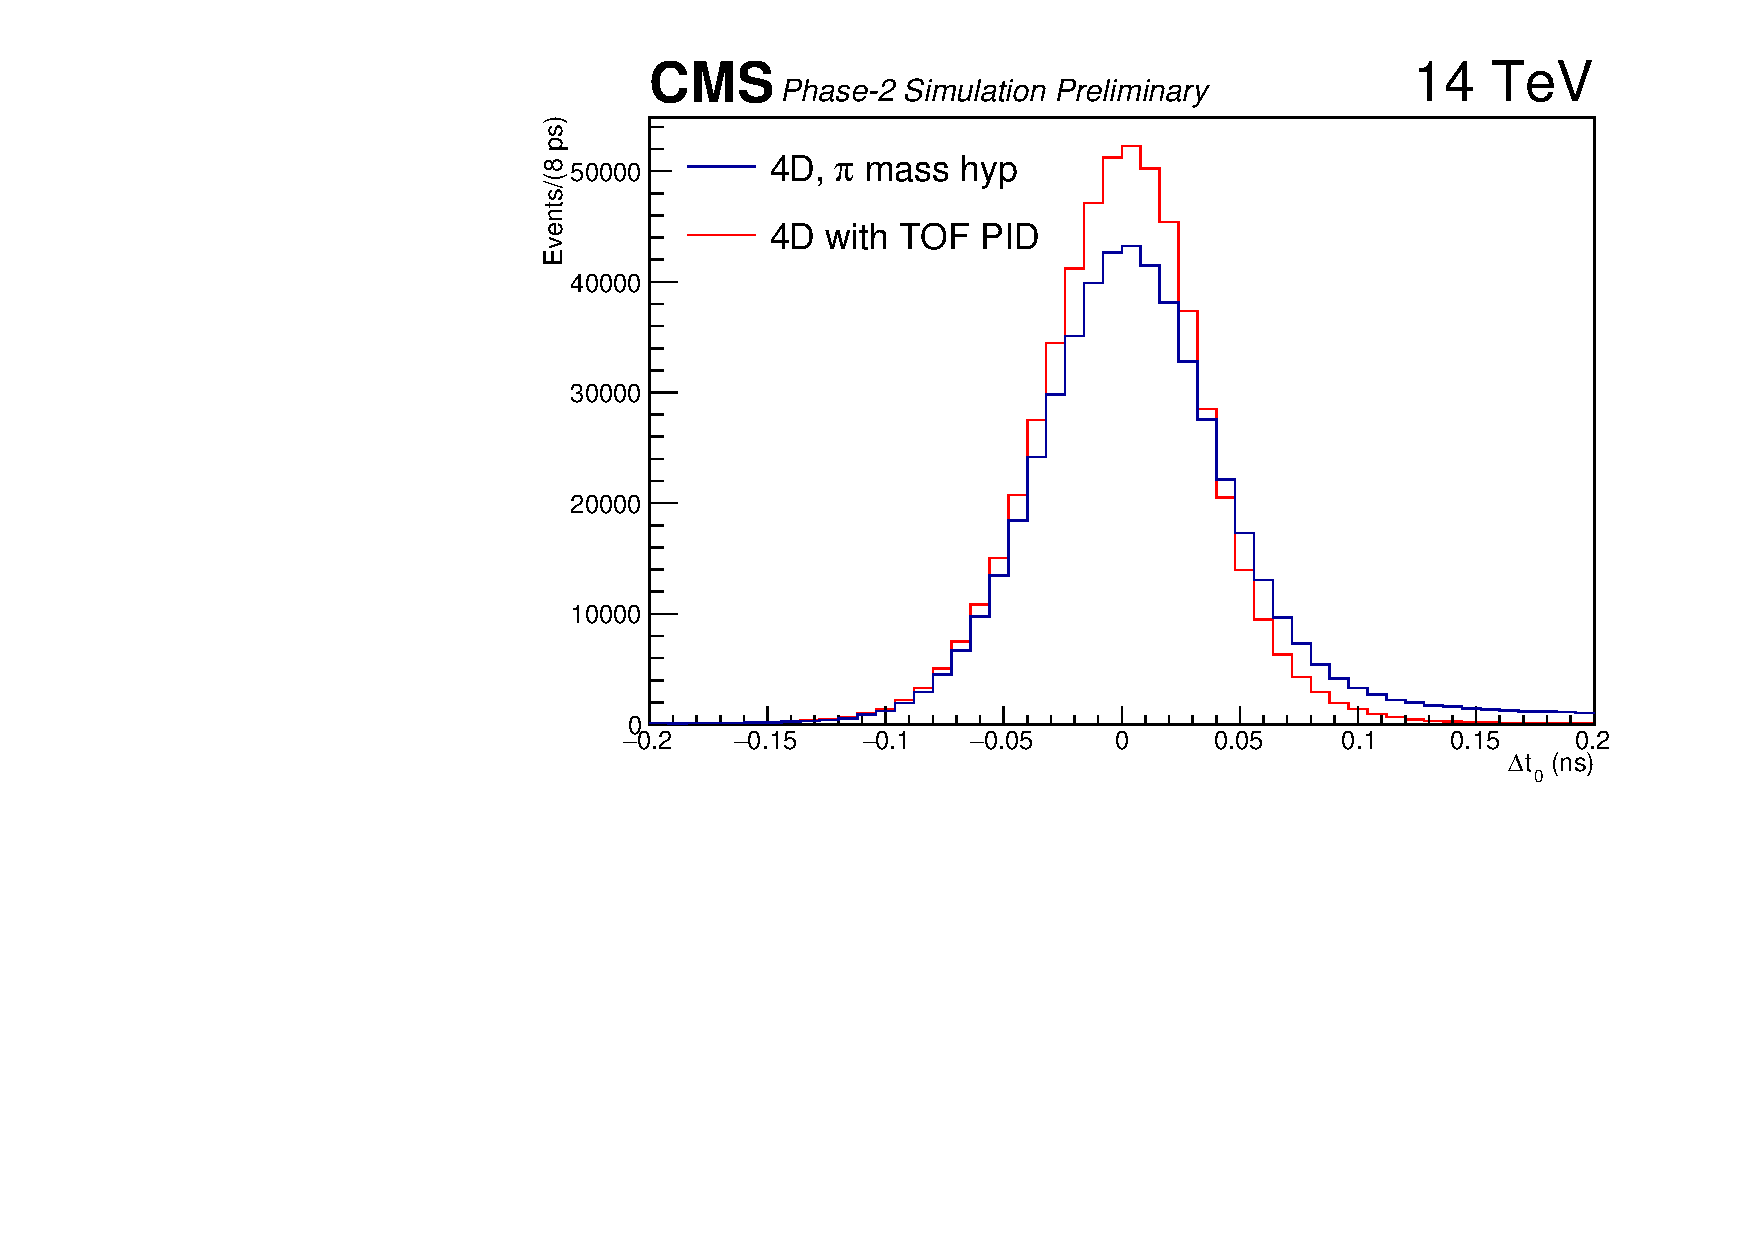
\includegraphics[width=0.48\textwidth]{fig/performance/4dvtx/ttbarnopu/dttrkgen_nopu_prelim.pdf}
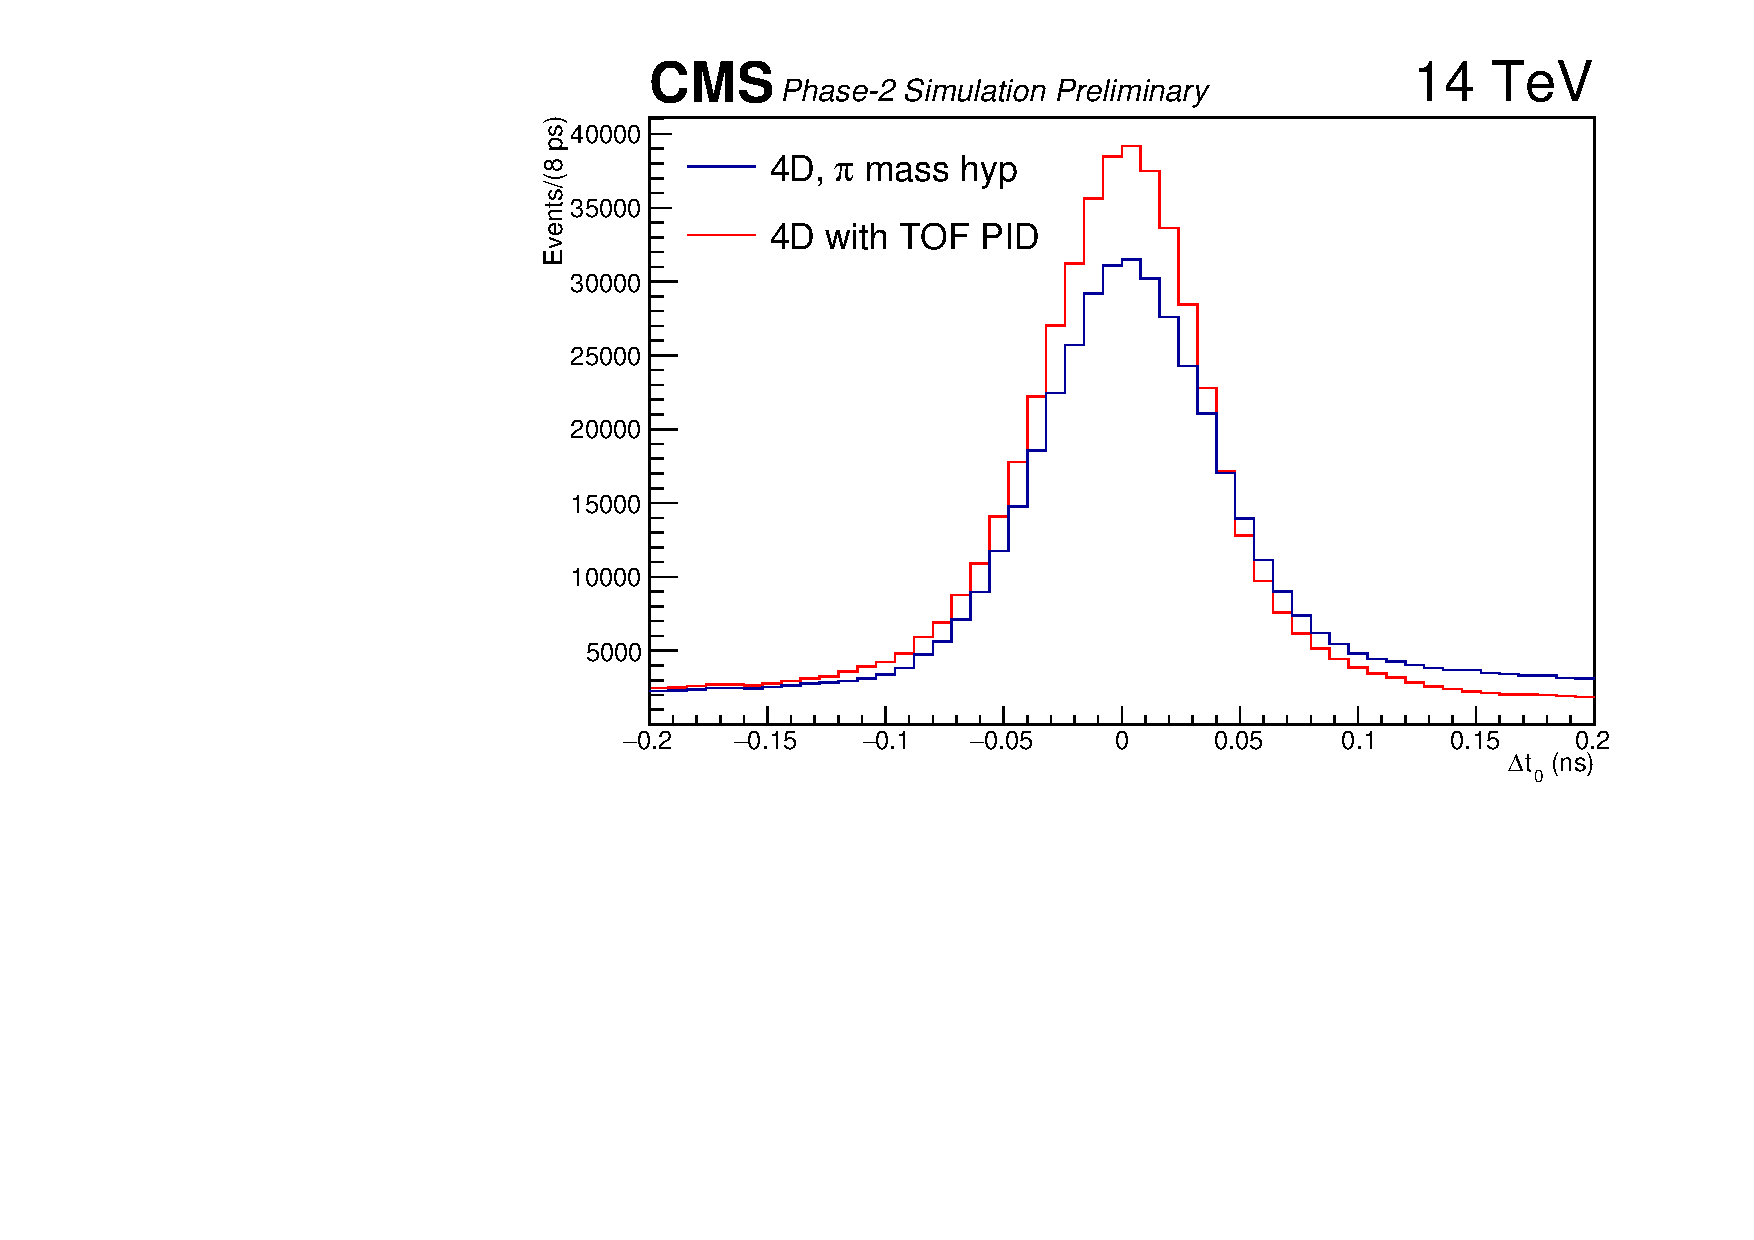
\includegraphics[width=0.48\textwidth]{fig/performance/4dvtx/ttbarpu200/dttrkgen_pu200_prelim.pdf}
\caption{Reconstructed time at the beamline with and without the use of time-of-flight particle ID for tracks reconstructed within $|\Delta z|<1$~mm of the generated hard interaction, in $t\bar t$ events with no pileup (left) and 200 PU (right).  The symmetric component of the tails in the pileup case include some tracks from pileup interactions which are reconstructed within 1~mm of the hard interaction.}
\label{fig:pidtres}
\end{figure}
